De manera análoga al diseño anterior, se optó por los valores $k_p = 2$ y $k_i = 0,9$. En la Figura \ref{fig:bode_pi} se puede observar el diagrama de Bode a lazo abierto con sus respectivos márgenes de fase y ganancia.

\begin{figure}[H]
  \centering
  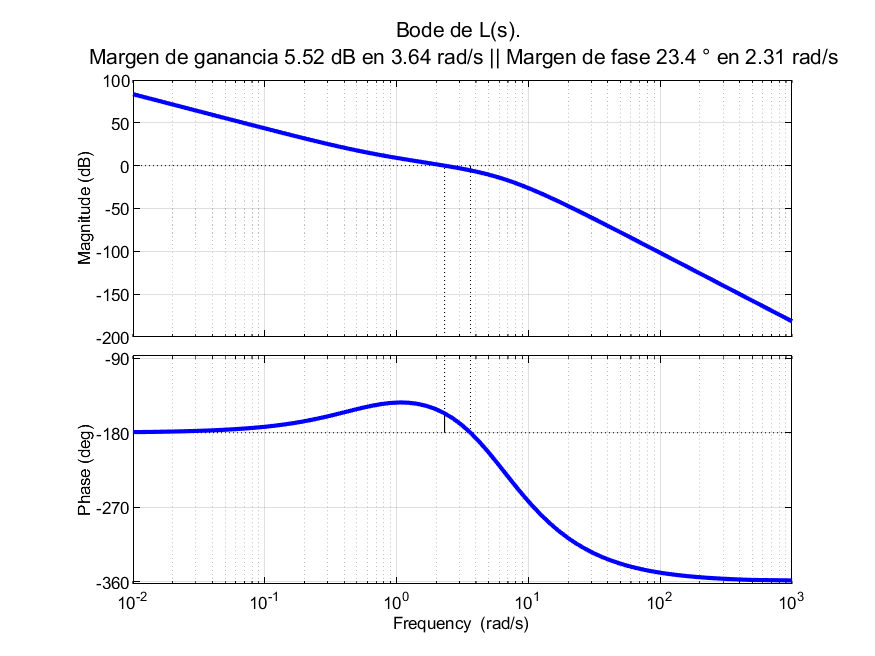
\includegraphics[width=0.75\textwidth]{img/PI/PI-Bode de L.png}
  \caption{Diagrama de Bode de $L(s)$.}
  \label{fig:bode_pi}
\end{figure}

En las Figuras \ref{fig:impulso_pi} y \ref{fig:escalon_pi} se observan las respuestas al impulso y al escalón a lazo cerrado medidas y simuladas, respectivamente. En las Figuras \ref{fig:control_impulso_pi} y \ref{fig:control_escalon_pi} se muestran sus respectivas acciones de control.

La acción integral del controlador PI acumula el error entre la referencia y la salida, aumentando o disminuyendo la acción de control mientras dicho error persista. De esta forma, aunque exista una desviación sostenida, el término integral continúa actuando hasta reducirla y hacer que la respuesta se acerque a la referencia. Esto se observa en los gráficos de acción de control: ante el impulso aparece una corrección rápida que luego disminuye a medida que el error se atenúa, mientras que ante el escalón la acción de control se ajusta de forma más sostenida hasta alcanzar el valor necesario para compensar el error en régimen permanente.

\begin{figure}[H]
  \centering
  \begin{minipage}{0.5\textwidth}
    \centering
    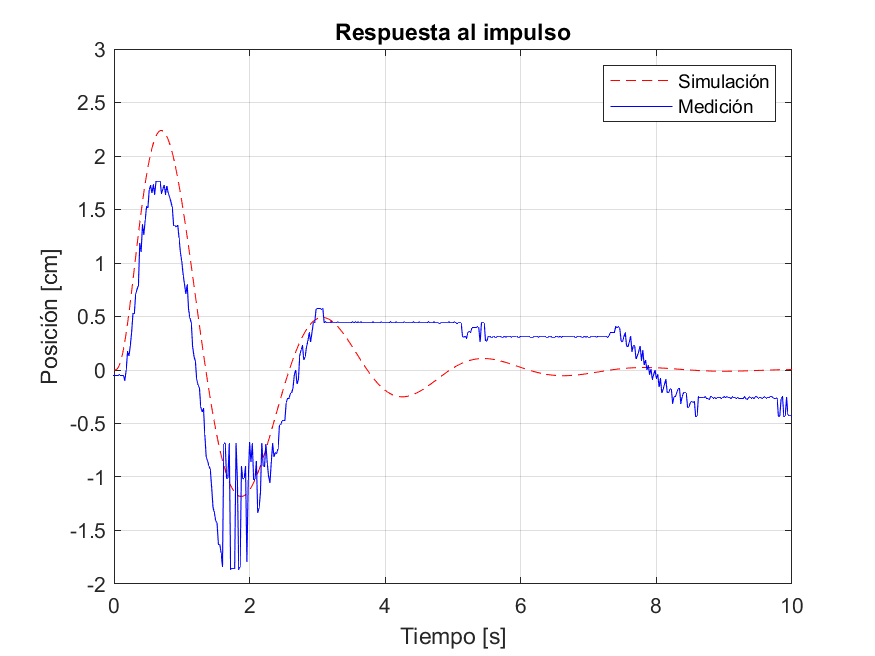
\includegraphics[width=\textwidth]{img/PI/PI-Respuesta al impulso.png}
    \caption{Respuesta al impulso de $T(s)$.}
    \label{fig:impulso_pi}
  \end{minipage}\hfill
  \begin{minipage}{0.5\textwidth}
    \centering
    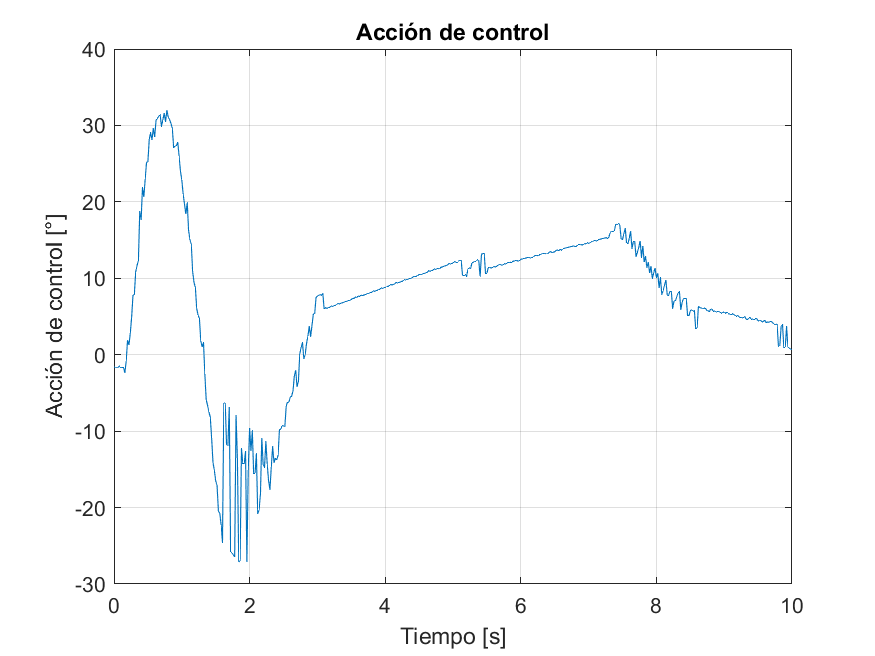
\includegraphics[width=\textwidth]{img/PI/PI-Acción de control(impulso).png}
    \caption{Acción de control ante impulso.}
    \label{fig:control_impulso_pi}
  \end{minipage}

  \vspace{0.4cm}

  \begin{minipage}{0.5\textwidth}
    \centering
    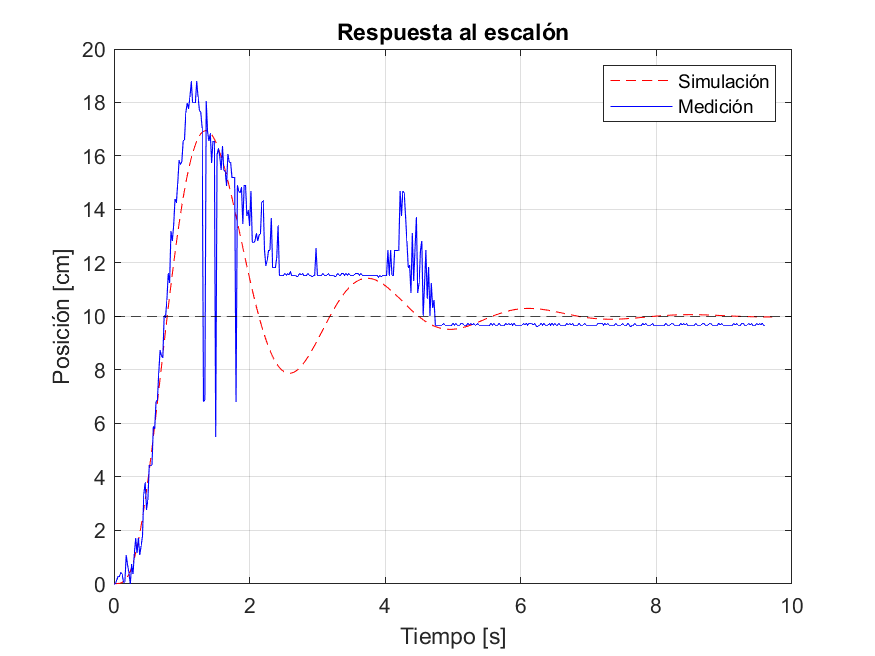
\includegraphics[width=\textwidth]{img/PI/PI-Respuesta al escalón.png}
    \caption{Respuesta al escalón de $T(s)$.}
    \label{fig:escalon_pi}
  \end{minipage}\hfill
  \begin{minipage}{0.5\textwidth}
    \centering
    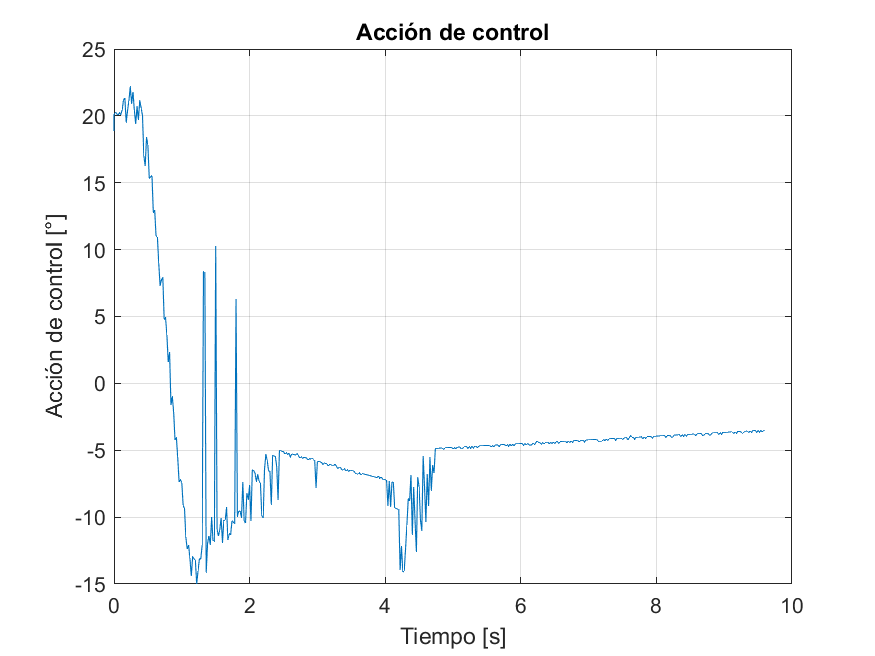
\includegraphics[width=\textwidth]{img/PI/PI-Acción de control(escalón).png}
    \caption{Acción de control ante escalón.}
    \label{fig:control_escalon_pi}
  \end{minipage}
\end{figure}